\documentclass[11pt]{article}

\usepackage[]{todonotes}
\usepackage{times}
\usepackage{fullpage}
\usepackage[pdfborder=false]{hyperref}
\usepackage{tabularx}
\usepackage{tabulary}
\usepackage{amssymb}

\usepackage{tikz}
\usetikzlibrary{trees}

% Enumeration environment: 1 -> 1.1 -> 1.1.1, etc
\makeatletter
\renewcommand{\labelenumii}{\arabic{enumi}.\arabic{enumii}}
\renewcommand{\labelenumiii}{\arabic{enumi}.\arabic{enumii}.\arabic{enumiii}}
\renewcommand{\theenumiii}{\arabic{enumiii}}
\renewcommand{\p@enumiii}{\arabic{enumi}.\arabic{enumii}.}
\makeatother

\setlength{\parindent}{0pt}
\setlength{\parskip}{11pt plus 3pt minus 2pt}

\begin{document}


%------------------------------------------------------------------------------- 

\title{Columbia AEHS\\Software Project Management Plan}
\author{Ben Straub\\Initech Corporation}
\date{Version 2.0\\5/10/2009}
\maketitle
\thispagestyle{empty}

The Advanced E-Healthcare System (AEHS) is the next step in Columbia Healthcare Group's (CHG)
technology strategy.  The system is to support healthcare provisioning, authorized access and
maintenance of patient records, orders, bills and other healthcare data, and integration among
Columbia's healthcare provider services including Columbia's recently deployed Claims Processing
System (CPS).

\vskip 1cm
{\Large \bf Revision History}

\begin{center}
  \begin{tabulary}{\textwidth}{c|L|l|l}
    \bf{Version} & \bf{Description}                     & \bf{Responsible Party} & \bf{Date} \\
    \hline \hline
    1.0          & Initial version of SPMP for review   & Ben Straub             & 4/19/2009 \\
    2.0          & Initial WBS and schedule             & Ben Straub             & 5/10/2009 \\
    3.0          & Managerial and Support Process Plans & Ben Straub             & 5/31/2009
  \end{tabulary}
\end{center}

\vskip 1cm
{\Large \bf Approval History}

\begin{center}
  \begin{tabulary}{\textwidth}{c|L|l|l}
    \bf{Version} & \bf{Description}      & \bf{Responsible Party} & \bf{Date} \\
    \hline \hline
    1.0          & Assignment 1 accepted & Kal Toth               & 4/19/2009 \\
    2.0          & Assignment 2 accepted & Kal Toth               & 5/10/2009
  \end{tabulary}
\end{center}
\clearpage

%-------------------------------------------------------------------------------
\tableofcontents
\clearpage


%-------------------------------------------------------------------------------
\section{Overview and Project Summary}

The AEHS project will provide Columbia Healthcare Group with a state-of-the-art information
management system.  AEHS will provide instant access to patient and clinician records from a variety
of environments, and will do so in a secure, user-friendly way.


\subsection{Purpose, Context, Scope of Requirements, and Objectives}

\subsubsection{Purpose}
The primary purpose for this project is to develop and deliver the AEHS system as specified by CHG.

\subsubsection{Context}
The key stakeholders for this project are:
\begin{itemize}
\item CHG management
\item Initech management
\item CHG IT staff, including CPS-specific staff
\item CHG users
\end{itemize}

\subsubsection{Scope}
The primary top-level requirements for this project are:
\begin{itemize}
\item Provide user interfaces for several categories of service:
  \begin{itemize}
  \item User workstations for healthcare workers
  \item External services and transactions
  \item Claims services, integrating with CPS
  \item System administration
  \end{itemize}
\item Securely store and provide access to several categories of information:
  \begin{itemize}
  \item Patient records
  \item Clinician information
  \item Healthcare knowledge base
  \item Billing records
  \end{itemize}
\end{itemize}


\subsubsection{Objectives}
The primary objectives of this project are:
\begin{itemize}
\item To deliver the AEHS system as specified and on schedule.
\item To allow the resulting system to be productized.
\end{itemize}


\subsubsection{Flexibility Matrix}
\newcolumntype{Y}{>{\centering\arraybackslash}X}
\begin{center}
  \begin{tabularx}{0.95\textwidth}{|l@{\hspace{0.5cm}}|Y|Y|Y|}
    \hline
    \bf Dimension                      & \bf Fixed  & \bf Constrained & \bf Flexible \\
    \hline \hline
    Delivery Schedule                  &            &                 & \checkmark   \\ \hline
    Project Cost                       & \checkmark &                 &              \\ \hline
    Requirements: Web UI               &            & \checkmark      &              \\ \hline
    Requirements: Mobile UI            &            & \checkmark      &              \\ \hline
    Requirements: Integration with CPS & \checkmark &                 &              \\ \hline
    Requirements: HIPAA compliance     & \checkmark &                 &              \\ \hline
    Requirements: Knowledge Base       &            &                 & \checkmark   \\ \hline
  \end{tabularx}
\end{center}


\subsection{Assumptions, Constraints and Dependencies}

Assumptions that underlie this plan include:

\begin{itemize}
\item Staff members of the appropriate skill set will be available when they are needed, and turnover
  will be no higher than 10\% per year.
\item It is possible to hire specialists with domain knowledge within time and budget constraints,
  and they will stay on this project until no longer needed.
\item Some of the experienced Initech staff will be available to act as development team leads.
\end{itemize}

The major constraints on this project are:

\begin{itemize}
\item The schedule and budget for this project are contractually fixed.
\item AEHS will integrate with an existing system for which no substitution is possible.
\end{itemize}

This plan has several external dependencies:

\begin{itemize}
\item CHG engineers are scheduled to be included in the development team for part of the project.
  There is a risk that these engineers won't be available, or will not be competent.
\item Access to the existing CPS is limited, and there is a risk that this access will be
  unavailable when it is needed.
\end{itemize}

\subsection{Project Deliverables}
This project's deliverables are:

\begin{itemize}
\item Plans
  \begin{itemize}
  \item Software Project Management Plan (SPMP)
  \item Software Requirements Plan (SRP)
  \item Software Development Plan (SDP)
  \item Software Test Plan (STP)
  \item Software Quality Assurance Plan (SQAP)
  \item Software Configuration Management Plan (SCMP)
  \end{itemize}
\item Technical Documents and Software
  \begin{itemize}
  \item Software Requirements Specification (SRS)
  \item Software Architecture and Design Document (SADD)
  \item Software Test Description(s) (STD)
  \item Software Test Report(s) (STR)
  \item Software User Manual(s) (SUM)
  \item Source Code
  \item Master and Backup CDs with Run-time, install, and read-me instructions
  \end{itemize}
\item Regular reports and progress documentation
  \begin{itemize}
  \item Progress reports and burn-down charts as dictated by development process
  \item Manual test run reports
  \item Weekly metrics: Source code, automated tests, and static analysis
  \end{itemize}
\end{itemize}


\subsection{Summary of Schedule and Budget}
The project budget includes 360 staff-months at \$10,000 per staff-month, for a total of
\$3,600,000.  Not included in the budget is the cost of additional equipment necessary for the
project, such as servers -- these items are billed directly to the customer.

The project schedule is 18 months, with the following milestones:

\begin{center}
  \begin{tabulary}{\textwidth}{L|l}
    \bf{Item}                    & \bf{Date}             \\
    \hline \hline
    Specification delivery       & 3/31/2009             \\
    Plan delivery                & 4/30/2009             \\
    Architecture/design delivery & 5/30/2009             \\
    Incremental builds           & every other Wednesday \\
    Final delivery deadline      & 7/1/2010
  \end{tabulary}
\end{center}


\subsection{Evolution of this SPMP}
This document will be revised periodically over the course of the project to record progress, such
as actual dates for deliverables, and to distribute information about changes in projected schedule
and plan.  In this case, ``periodically'' means at every major milestone.  These changes will be
managed by requiring each release to be approved by the change control board.



%-------------------------------------------------------------------------------
\section{References}
\begin{itemize}
\item AEHS Terms of Reference
\item AEHS Project Contract
\item IEEE 1058 -- Standard for Software Project Management Plans
\item Initech Acceptance Procedure
\end{itemize}


%-------------------------------------------------------------------------------
\section{Definitions}
\begin{description}
\item[CHG] Columbia Healthcare Group
\item[AEHS] Advanced E-Healthcare System
\item[CPS] Claims Processing System
\end{description}



%-------------------------------------------------------------------------------
\section{Project Organization}
\subsection{Organizational Interfaces (Internal and External)}
The project organization chart looks something like this:

\begin{center}
  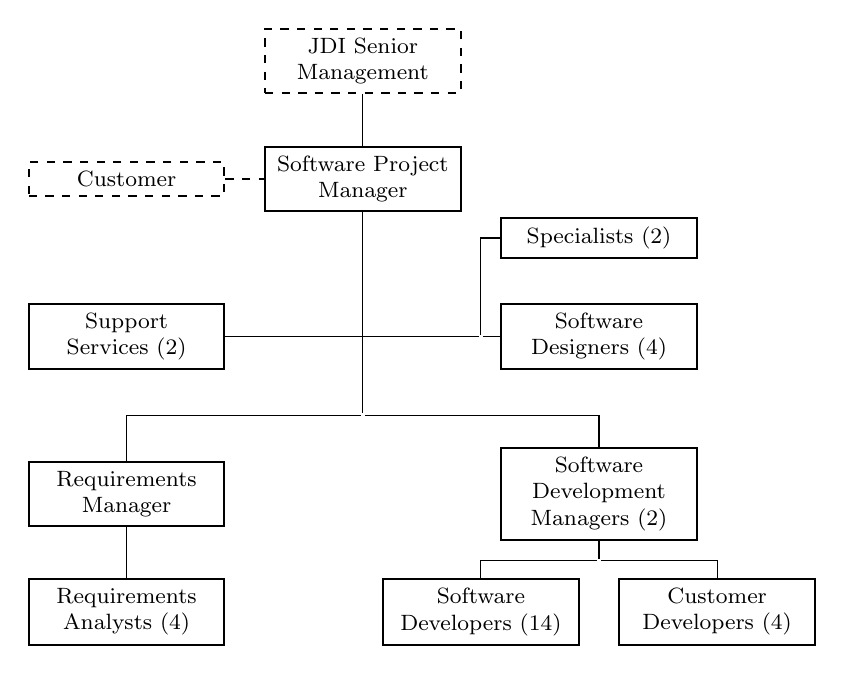
\begin{tikzpicture}
    \tikzstyle{box}=[draw, rectangle, thick, font=\footnotesize, text centered, text width=2.25cm];
    \tikzstyle{empty}=[inner sep=0];

    \node[box,dashed] at (0,0) (mgmt)  {JDI Senior Management};
    \node[box,dashed] at (-3,-1.5) (cust)  {Customer};
    \node[box] at (0,-1.5) (spm)   {Software Project Manager};
    \node[box] at (3, -2.25) (spec) { Specialists (2) };
    \node[empty] at (1.5,-3.5) (junct) {};
    \node[box] at (3, -3.5) (des) {Software Designers (4)};
    \node[box] at (-3, -3.5) (sup) {Support Services (2)};
    \node[empty] at (0, -4.5) (junct2) {};
    \node[box] at (-3, -5.5) (rqm) {Requirements Manager};
    \node[box] at (-3, -7) (rqa) {Requirements Analysts (4)};
    \node[box] at (3, -5.5) (sdm) {Software Development Managers (2)};
    \node[empty] at (3, -6.35) (junct3) {};
    \node[box] at (1.5, -7) (dev) {Software Developers (14)};
    \node[box] at (4.5, -7) (cus) {Customer Developers (4)};

    \draw [dashed] (cust) -- (spm);
    \draw (mgmt) -- (spm)
          (spm) |- (junct)
          (junct) |- (spec)
          (junct) -- (des)
          (junct) -- (sup)
          (spm) -- (junct2)
          (junct2) -| (rqm)
          (junct2) -| (sdm)
          (rqm) -- (rqa)
          (sdm) -- (junct3)
          (junct3) -| (dev)
          (junct3) -| (cus);

    % \tikzstyle{every node}=[rectangle, minimum width=1.25in, draw, thick, font=\footnotesize]
    % \tikzstyle{level 1}=[level distance=1.75in]
    % \tikzstyle{level 2}=[level distance=1.5in, sibling distance=20pt]

    % \node {Project Manager}[edge from parent fork right, grow=right]
    % child {node {QA Manager}
    %   child {node {Testers}}
    %   child {node {Config Mgmt}}}
    % child {node {Requirements Mgr}
    %   child {node {Analysts (4)}}}
    % child {node {Specialists (2)}}
    % child {node {Support (2)}}
    % child {node {Development Mgrs (2)}
    %   child {node {Team D}}
    %   child {node {Team C}}
    %   child {node {Team B}}
    %   child {node {Team A}}};
  \end{tikzpicture}
\end{center}

The SPM acts as a bridging node for all the functional teams in the project, and is also the primary
point of contact for the customer at a project level.  





\subsection{Project Roles and Responsibilities}

{\bf Project Management} -- The SPM is responsible for the maintenance of this plan, as well as
monitoring the rest of the team for project health and progress.

{\bf Support} -- Two general support staff and two domain specialists, all of whom report to the
SPM.  These staff act as shared resources, and are available to any of the other sub-teams as
necessary.

{\bf Requirements} -- Four analysts, who report to a single manager.  The manager reports directly
to the SPM.

{\bf Architecture} -- The architecture and design of the system will be developed by the development
team.  The designated architect is responsible for maintaining conceptual integrity and the product
vision, but is otherwise just another member of the development team.

{\bf Development} -- The development organization consists of four teams of 4-5 developers.  Each
team consists of a lead, a CHG engineer, and several other staff engineers to fill out the team.
The development team as a whole is supported by two managers, who are responsible for smoothing
communication and other issues, and aggregating information for the SPM.

{\bf QA/Test/CM} -- A single QA manager oversees several {\bf (TBD)} full-time testers, as well as a
dedicated configuration management engineer.  The QA manager is also responsible for ensuring the
project team follows specified procedures and processes.



%-------------------------------------------------------------------------------
\section{Managerial Process}

\subsection{Work Breakdown and Tasks}

\subsubsection{Work Breakdown}

\begin{enumerate}
\item Manage Project
  \begin{enumerate}
  \item Initiate project
  \item Conduct project
  \item Closeout project
  \end{enumerate}
\item Do System Analysis
  \begin{enumerate}
  \item Develop Requirements
  \end{enumerate}
\item Develop Software
  \begin{enumerate}
  \item Prototype Application Service UIs
    \begin{enumerate}
    \item \label{wbs:pre1} Develop UI concept
    \item \label{wbs:task} Develop working UI prototype
    \item \label{wbs:post1} Refinement I
    \item Refinement II
    \item Produce requirements specification
    \end{enumerate}
  \item Prototype Technology UIs
  \item Develop System Architecture and High-Level Design
  \item Develop Foundation Software
  \item Develop Application Server Functions
  \item Acquire Appointments/Forms Components
  \end{enumerate}
\item Verify System
  \begin{enumerate}
  \item Develop test plan
  \item Develop test procedures
  \item Perform Integration Testing
  \end{enumerate}
\item Validate System
  \begin{enumerate}
  \item Perform traceability analysis
  \end{enumerate}
\item Perform CM
  \begin{enumerate}
  \item Keep documents in version control
  \item Manage changes to baselined documents
  \end{enumerate}
\item Prepare Technical Publications
  \begin{enumerate}
  \item Develop user documentation
  \item Develop training materials
  \end{enumerate}
\item Deliver System
  \begin{enumerate}
  \item Select and Evaluate Site Hardware
  \item Install Site Hardware
  \item Deploy Software at Sites
  \item Perform user training
  \end{enumerate}
\end{enumerate}


\subsubsection{Work Packages}

\begin{tabular*}{\textwidth}{l@{\hspace{1cm}}l}
  \hline
  Task identifier:        & \ref{wbs:task} Develop working UI prototype                              \\
  Task description:       & Design and implement a mock-up of the UI concept.                        \\
  Estimated duration:     & 2 weeks                                                                  \\
  Resources needed:       &                                                                          \\
  \hspace{1em} Personnel: & 3 developers, 1 customer engineer                                        \\
  \hspace{1em} Skills:    & HTML/CSS/JavaScript development                                          \\
  \hspace{1em} Tools:     & Workstations, source control                                             \\
  \hspace{1em} Travel:    & None                                                                     \\
  Predecessor tasks:      & \ref{wbs:pre1}                                                           \\
  Successor tasks:        & \ref{wbs:post1}                                                          \\
  Work products:          & Functional UI prototype                                                  \\
  Baselines created:      & None                                                                     \\
  Risk factors:           & Prototyping activities are inconclusive.                                 \\
  Acceptance criteria:    & Concept is implemented, prototype is functional enough to show to users. \\
  \hline
\end{tabular*}

\subsection{Dependencies}

\begin{enumerate}
\item The prototyping tasks need to be done before the requirements can be finalized, and thus
  before the final implementation can be performed.
\item Server implementation for a particular function must be complete before integration testing
  for that function can commence.
\item Development must be complete before acceptance testing can start.
\end{enumerate}


\subsection{Resources}

\begin{center}
  \begin{tabular}{l@{\hspace{1cm}}|l|l}
    \bf Task                             & \bf Resource          & \bf Months \\
    \hline \hline
    1. Manage Project                    & SPM                   & 1-18       \\
    2. Do System Analysis                & Requirements Analysts & 1-8        \\
    3.1 Prototype Application Service UI & Dev. Team A           & 3-6        \\
    3.2 Prototype Technical UI           & Dev. Team A           & 7-10       \\
    3.3 Develop System Architecture      & Software Designers    & 3-6        \\
    3.4 Develop Foundation Software      & Dev. Team B           & 3-6        \\
    3.5 Develop Server Functions         & Dev. Team C           & 5-11       \\
    3.6 Acquire Appointments/Forms COTS  & Dev. Team A           & 9-12       \\
    4. Verify System                     & QA Team               & 12-15      \\
    5. Validate System                   & QA Manager            & 1-18       \\
    6. Perform CM                        & Configuration Manager & 1-18       \\
    7. Prepare Technical Publications    & Dev. Managers         & 1-18       \\
    8.1 Select and Evaluate Site HW      & Dev. Team C           & 3-4        \\
    8.2 Install Site HW                  & Dev. Team C           & 16-17      \\
    8.3 Deploy SW at Sites               & Dev. Team C           & 18         \\
    8.4 Perform User Training            & Dev. Team A           & 15-18      \\
  \end{tabular}
\end{center}

\subsection{Budget and Resource Allocation}

\begin{center}
  \begin{tabular}{l@{\hspace{1cm}}l@{\hspace{1cm}}r}
    \bf Task                             & \bf Assignment          & \bf Person-weeks \\
    \hline \hline
    1. Manage Project                    & 1 SPM                   & 72               \\
    2. Do System Analysis                & 4 Rq. Analysts, 1 Mgr   & 120              \\
    3.1 Prototype Application Service UI & Dev. Team A (3)         & 48               \\
    3.2 Prototype Technical UI           & Dev. Team A (3)         & 48               \\
    3.3 Develop System Architecture      & 4 SW Designers          & 64               \\
    3.4 Develop Foundation Software      & Dev. Team B (6)         & 96               \\
    3.5 Develop Server Functions         & Dev. Team C (5)         & 140              \\
    3.6 Acquire Appointments/Forms COTS  & Dev. Team A (3)         & 48               \\
    4. Verify System                     & 4 Testers               & 140              \\
    5. Validate System                   & 1 QA Manager            & 8                \\
    6. Perform CM                        & 1 Configuration Manager & 64               \\
    7. Prepare Technical Publications    & 2 Dev. Managers         & 128              \\
    8.1 Select and Evaluate Site HW      & Dev. Team C (5)         & 40               \\
    8.2 Install Site HW                  & Dev. Team C (5)         & 40               \\
    8.3 Deploy SW at Sites               & Dev. Team C (5)         & 20               \\
    8.4 Perform User Training            & Dev. Team A (3)         & 48               \\
    \hline
                                         &                         & \bf 1,124        \\
    \cline{3-3}
  \end{tabular}
\end{center}

With an average loaded cost of \$2,400, this gives a total cost estimate of \$3,021,312.


\subsection{Schedule}
\todo[inline]{Uncomment this for PDF version.}
% \includegraphics[width=\textwidth]{gantt.png}



\subsection{Monitoring, Reporting, and Control Mechanisms}
\todo[inline]{Describe what progress and control metrics you will use to report progress across your
  teams, to senior management and to the customer.  What will be included in your reports?  How
  often will you deliver them and brief various stakeholders?}
\subsection{Requirements Management and Control}
\todo[inline]{One key risk is that the scope of the work may be larger than originally anticipated.
  Briefly describe your approach for monitoring possible “scope creep” and negotiating required
  changes with the customer and your senior management.}
\subsection{Risk Management}
\todo[inline]{For each project risk, what do you plan to do to mitigate the risk?  For example, what
  if your customer does not deliver certain documents or tools?  What if your sponsor drops out or
  does not provide as much guidance as you were hoping?  What if a key member of your team drops
  out, how will you cover this loss?  What if after some initial work you discover that there is
  more work than you thought?  How will you deal with this but still achieve a reasonable outcome?
  What can you do to prepare for such eventualities?}




%-------------------------------------------------------------------------------
\section{Technical Processes}
\subsection{Process Model}
This project will make use of several process models during various phases of the project.

An evolutionary model will be used for feasibility and exploration of requirements in
lesser-understood areas of functionality.  As the requirements for these areas firm up, evolutionary
and prototyping activities will phase out.  The endpoint of these activities is the Specification
Delivery milestone, which consists of the SRS v1.0 baseline.

Most of the requirements elicitation and architecture phases of the project will follow something
like a waterfall model.  These activities must be mostly complete before detailed design and
implementation can proceed.  The Plan Delivery milestone is the endpoint of these activities, and
includes delivery of v1.0 baselines of the SPMP, SRP, SDP, STP, SQAP, and SCMP, as well as an
updated version of the SRS.

The architecture, design, and implementation of the system will be delivered in an incremental
fashion, with deliveries every other Wednesday.  Four increments (starting with the Specification
Delivery milestone) will be dedicated to the overall architecture of the system, as well as some
high-level design, culminating in the Architecture/Design Delivery milestone.  Detailed design and
implementation will be performed during the remaining increments.

Once the architecture and detailed design are mostly complete, most of the development effort will
follow an incremental model, with testable requirements-subset releases available every two weeks.
Full integration and acceptance testing will be performed on most of these releases in order to
prevent a test-fix-release crunch late in the project schedule.

\todo{Draw a picture?}


\subsection{Methods, Tools and Techniques}
Architecture and design specification will make use of UML for diagrams, though most of the
specification will be in prose.  Some portions may make use of a formal mathematical notation to
avoid ambiguity and prevent defects.

Source code will be stored in source control, and will follow coding style guidelines.  A continuous
integration build system will be used, with a dashboard visible to all team members.  Release
building and deployment will be automated as much as possible, to facilitate semiweekly releases and
testing.  A defect tracking tool will be used, and the customer will have full access.

Automated unit testing will be used extensively, especially on components which are relied upon by
other software modules.  Wherever possible, the acceptance tests will be automated as well, to
ensure that they are run as often as possible.



\subsection{Development Environment and Infrastructure}
Each developer is free to choose his or her own OS and tools, but project management will ensure
that reasonable commercial tools are available for use if they are significantly better than free
alternatives.  Each developer will have exclusive use of at least one workstation and two test
machines.  Developers working on mobile interfaces will also have exclusive use of two targeted
mobile devices.

The primary platform for the server-side subsystems will be the JVM.  Development teams are free to
use any language that runs on that platform, so long as the selection of tools does not adversely
affect the architecture or design of the system as a whole, or interaction with other subsystems.

The system is required to integrate with the existing CPS system, so it will be necessary to
replicate that system's behavior for development.  This will be accomplished by doing a local
deployment of that system with a dummy database.  If that approach is not feasible, the behavior of
that system will need to be replicated with a mock-up.

Source code management, issue tracking, and documents will be managed using the tools already in
place at Initech.


\subsection{Acceptance Process}
All hardware and software purchased for the purposes of this project will be run through the
standard Initech Acceptance Procedure.



%-------------------------------------------------------------------------------
\section{Support Processes}
\todo[inline]{Describe support processes for the following:}
\subsection{Software Configuration Management}
\todo[inline]{What will you do to ensure that you control versions of your documents and code?}
\subsection{Software Quality Assurance}
\todo[inline]{How will you ensure that your documents and code have been independently reviewed by
  someone on your team?}
\subsection{Documentation Management}
\todo[inline]{Describe how you will manage the key software documents produced by the project, in
  particular the SPMP, SRS, SAD, user documentation and other key customer deliverables.  How will
  you review, approve, and release these documents (what, who, how, when)?}
\subsection{Subcontractor Management}
\todo[inline]{Describe the work that will be contracted out, if any, deliverables, schedules for
  delivery, and subcontractor control mechanisms to be used to ensure timeliness and quality of
  deliverables.  }




%-------------------------------------------------------------------------------
\section{Additional Supporting Plans}
\textit{TBD}
% \todo[inline]{If required, additional plans can be inserted here.}




%-------------------------------------------------------------------------------
% \section{Annexes}
% \textit{TBD}
% \todo[inline]{These should include details that would clutter the main sections.  All items herein should be references from somewhere in the main body of the document.  }



\end{document}
